\section{Observation Study}\label{observational}

Our first study assessed a comparison to a baseline on a simple task; our second study sought to assess tasks that were less constrained and more complex. We asked participants to build up two kinds of augmentations where they had freedom in the precise outcome. We sought to understand (1) if could they learn enough of Delta to succeed (2) the appropriateness of the various language constructs.

\subsection{Methods}

\paragraph{Participants.}
Ten of the 19 participants from the controlled study (Section \ref{results}) took part in an observation study. We sampled in this way for convenience; we already knew these participants could pass our inclusion criteria. A consequence of this choice is that participants already had some small amount of training in Delta. In aggregate, participant backgrounds was very similar to the prior study: participants rated their comfort writing LaTeX formulas as a median of 4 on a 5-point Likert scale ($\sigma = 1.03$) and with JavaScript as a median of 3.5 ($\sigma = 1.43$). All had some prior experience with React. Below, we refer to participants by anonymized identifiers assigned to them during the study (e.g., P21, P48).

\paragraph{Setup.} Like the controlled study, these study sessions were held on Zoom with coding taking place in a GitHub Codespace.

\paragraph{Tasks.}

Each participant completed two open-ended formula authoring tasks, each lasting up to 30 minutes. In each task, participants were given an empty Delta config as a starting point, with placeholders for formulas, variables, and semantics. They were given a task sheet that provided the formula's LaTeX, background about the formula, an example scenario with concrete values, and questions that could motivate potential augmentation ideas. Participants were instructed to augment the formula in whatever way they thought best helped a reader understand the underlying concept; the task sheets stated ``there is no single right answer'' and encouraged participants to try alternatives. Task~2 additionally required that the augmentation include at least one step.

Tasks were chosen to test essential parts of the Delta language. Task 1 (T1) assessed the basic interaction and notation features, while Task 2 (T2) evaluated the stepping syntax. Graphing and SVG features were excluded to keep session length feasible (already ${\sim}$2 hours); they depended on features from T1 and T2, so we prioritized those features instead.
T1 required augmentation of a formula for radioactive decay formula $N(t) = N_0 \cdot e^{-\lambda t}$ and T2 a formula for expected value $E = \sum_{x \in X} x\, P(x)$. Prior to each task, participants followed a self-paced written tutorial introducing all features they might need for the task on an example formula. They were given 20 minutes.

% \vspace{0.5em}
% \noindent
% \fbox{\begin{minipage}[t]{0.44\columnwidth}
% \centering
% \textbf{T1:} \textit{Radioactive decay}
% \[N(t) = N_0 \cdot e^{-\lambda t}\]
% \end{minipage}}%
% \hfill
% \fbox{\begin{minipage}[t]{0.44\columnwidth}
% \centering
% \textbf{T2:} \textit{Expected value}
% \[E = \sum_{x \in X} x\, P(x)\]
% \end{minipage}}
% \vspace{0.5em}

% \noindent
% Both tasks provided starter code with imports in place and asked participants to fill in a Delta configuration---specifying formulas, variables, and semantics---to make the formula interactive. participants were given the relevant LaTeX as a starting point and were encouraged to augment the formula in whatever way they thought best helped a reader understand the underlying concept. Each task sheet included background on the formula, an example scenario with concrete values, and suggested questions for exploration.

% \vspace{0.5em}
% \noindent
% \fbox{\begin{minipage}[t]{0.44\columnwidth}
% \centering
% \textbf{T1:} \textit{Radioactive decay}
% \[N(t) = N_0 \cdot e^{-\lambda t}\]
% \end{minipage}}%
% \hfill
% \fbox{\begin{minipage}[t]{0.44\columnwidth}
% \centering
% \textbf{T2:} \textit{Expected value}
% \[E = \sum_{x \in X} x\, P(x)\]
% \end{minipage}}
% \vspace{0.5em}


\paragraph{Duration.}
Each task lasted up to 30 minutes, after which the facilitator stopped the author. Although tasks were open-ended with no fixed completion criteria, all ten participants produced a working interactive formula with correct computation and semantics and had time to iterate on its design. Including tutorials, questionnaires, and transitions, sessions lasted approximately 2 hours.

\paragraph{Measurement and Analysis.}
9 of 10 sessions were facilitated by the same researcher; 1 by a second researcher following the same protocol. Participants were told to think aloud, and the facilitator could interrupt with process questions. Post-task questionnaires after each task asked participants to rate usefulness, intuitiveness, and difficulty of Delta's main features on Likert scales and elaborate in free text. Because each task introduced different features, questionnaires asked only about features relevant to that task---basic interaction and notation for T1, stepping for T2. Both researchers independently reviewed recordings and compiled timestamped observation logs documenting feature usage patterns, error sequences, recovery strategies, and notable utterances. One researcher then performed qualitative coding across all data, identifying common workflows, design successes, and gaps. Retained codes were those lending insight into designing future DSLs like Delta.

\subsection{Results}

All ten participants completed both tasks within the allotted 30 minutes each.
% We report self-reported intuitiveness and difficulty ratings from the post-task questionnaires alongside qualitative observations from the think-aloud sessions. Figure~\ref{fig:obs-intuitiveness} summarizes the intuitiveness Likert-scale ratings for both tasks. Self-reported difficulty ratings followed a largely similar distribution and are included in the appendix (Figure~\ref{fig:obs-difficulty}).
We first describe design successes and then gaps. Design successes are organized using the Cognitive Dimensions of Notations framework~\cite{Blackwell2003-gv}, which provides a vocabulary for evaluating the usability of notational systems like DSLs. We foreground two dimensions that were central concerns in our design process: \emph{closeness of mapping} (how naturally the notation maps to the problem domain) and \emph{viscosity} (effort to make small changes).

\begin{figure}[t]
  \centering
  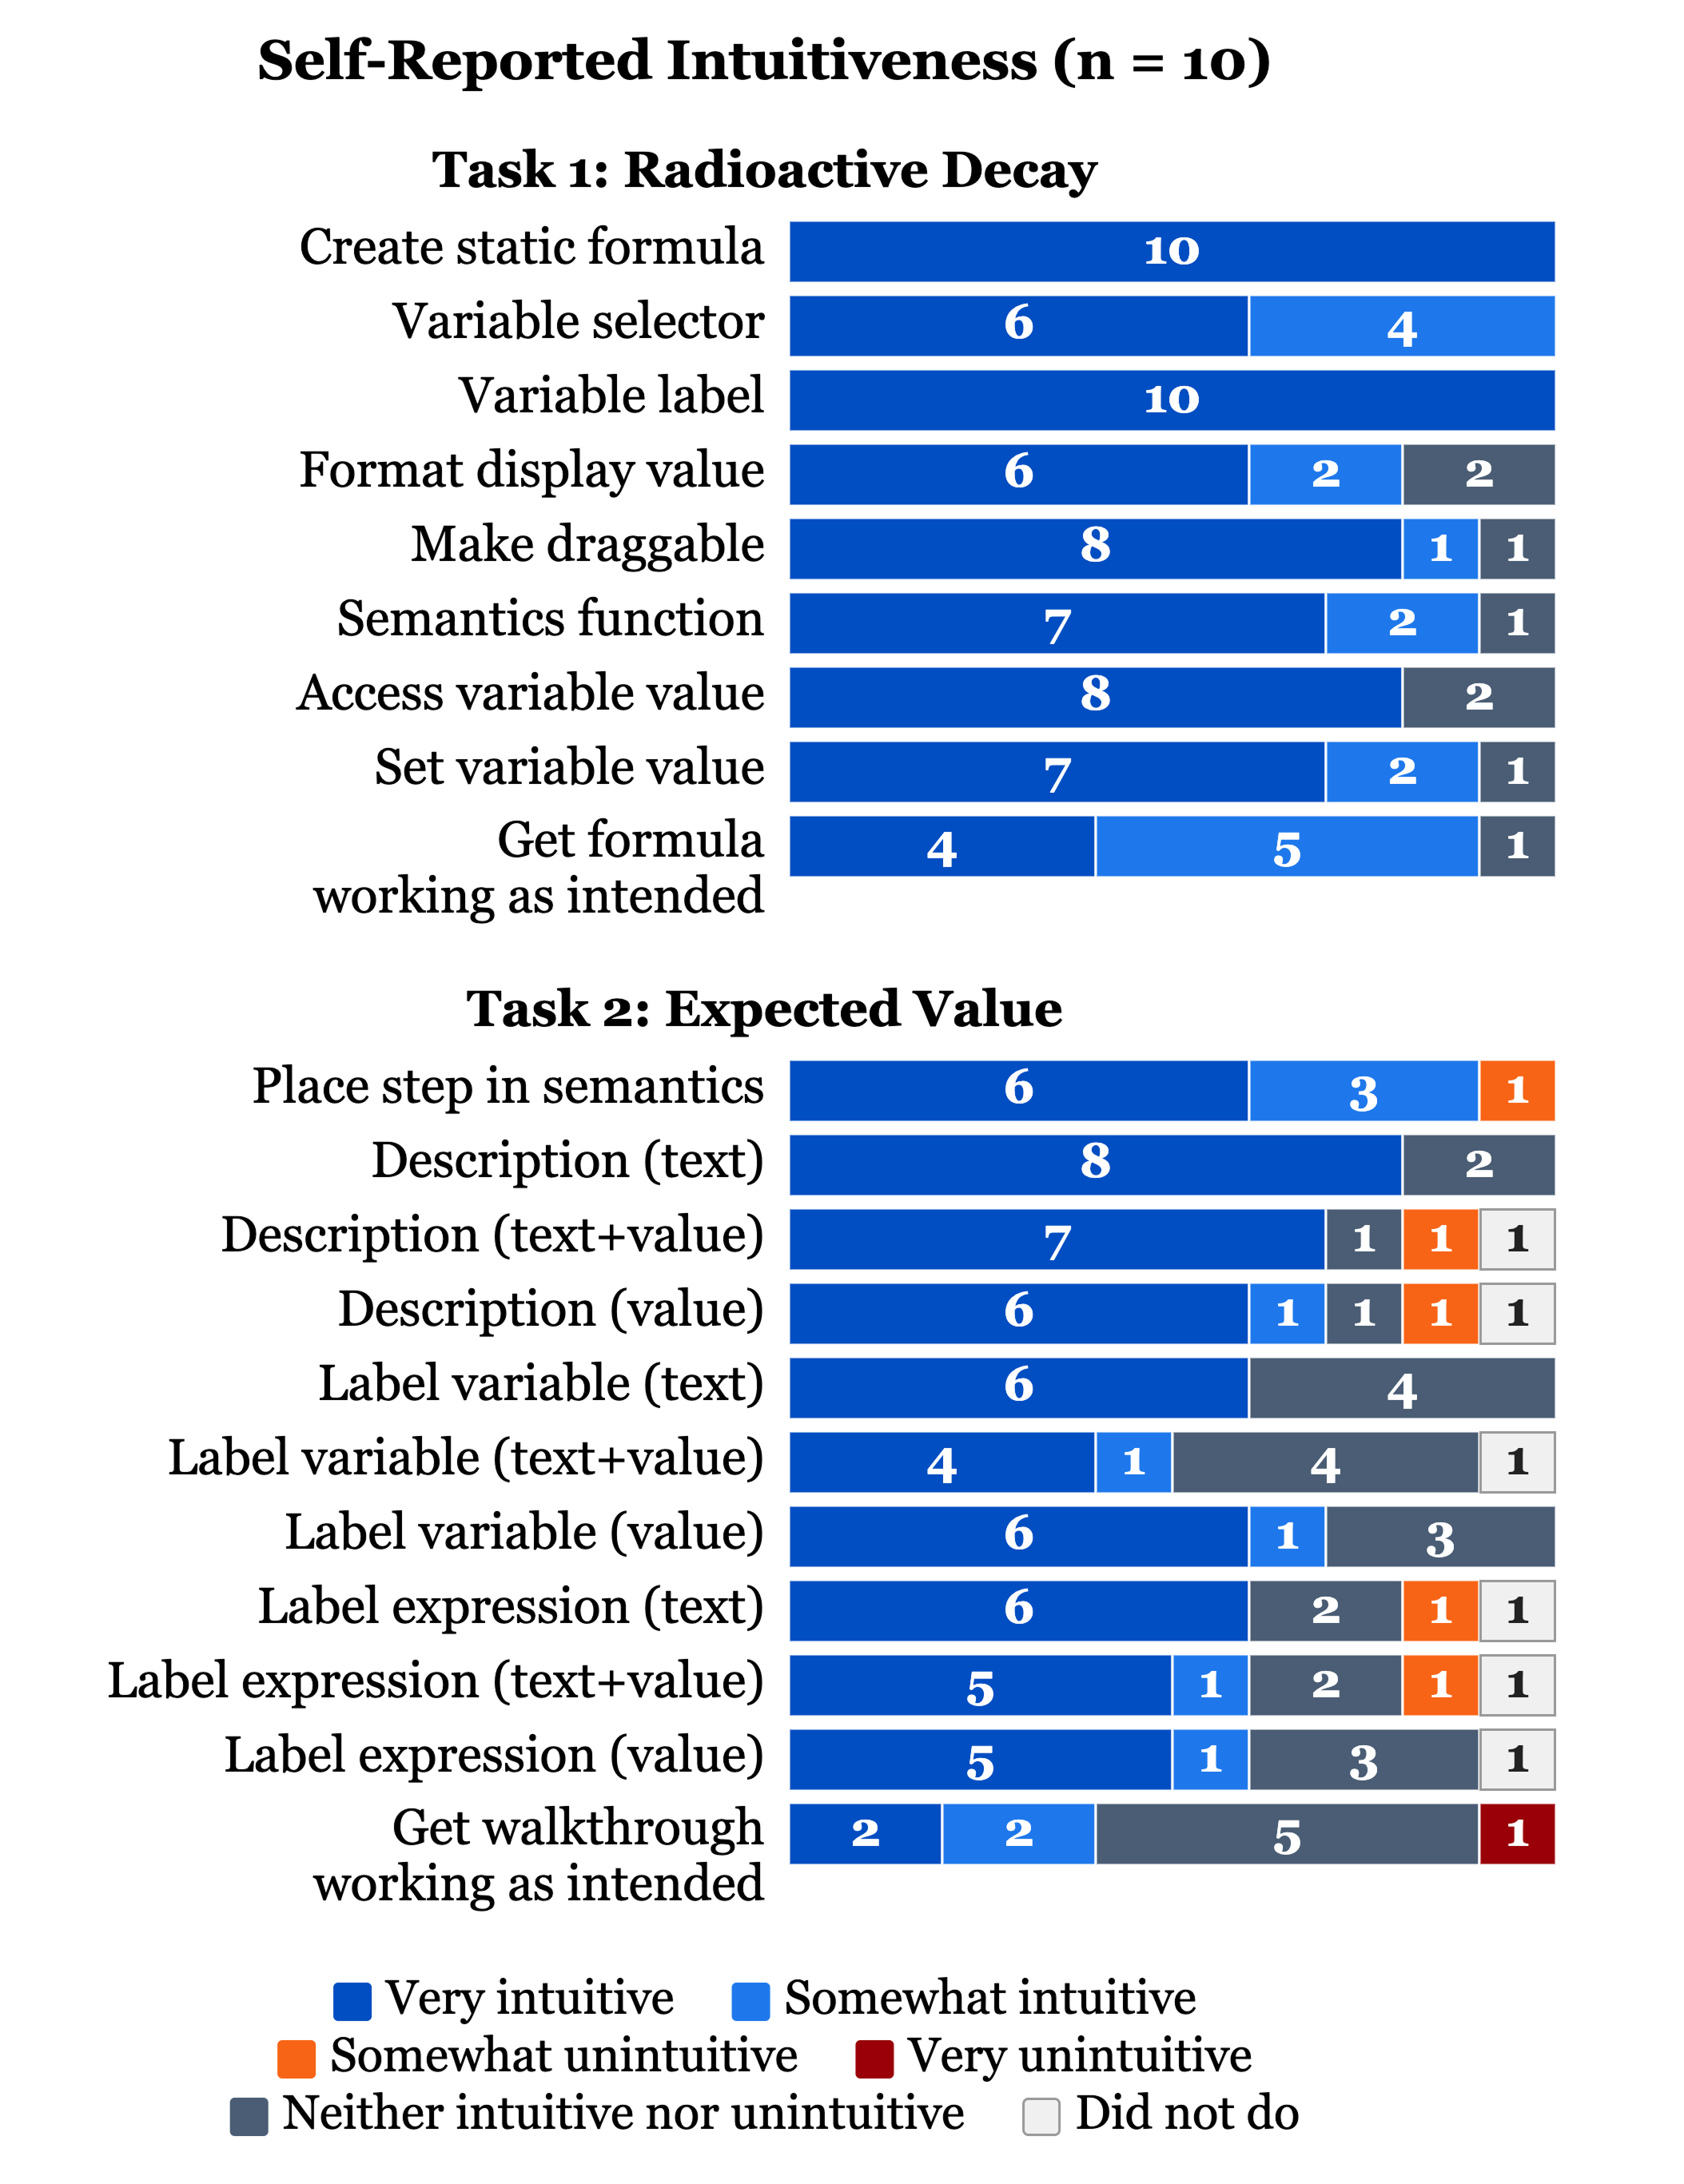
\includegraphics[width=\columnwidth]{fig/intuitiveness.png}
  \caption{\textbf{Self-reported intuitiveness ratings.} participants rated the intuitiveness of library features on a 5-point Likert scale ($n = 10$). Task~1 covers nine basic interaction and notation features; Task~2 covers eleven stepping features.}
  \Description{Diverging stacked bar chart showing Likert-scale intuitiveness responses for both tasks side by side. Most bars are dominated by blue (very intuitive / somewhat intuitive), with more spread visible for holistic items like getting the formula or walkthrough working as desired.}
  \label{fig:obs-intuitiveness}
\end{figure}

\subsubsection{Closeness of mapping}
All participants reported intuitiveness and difficulty of all language constructs and overall process for both tasks. Construct intuitiveness was our proxy for closeness of mapping; distributions of ratings appear in in Figure~\ref{fig:obs-intuitiveness}; difficult followed similar distributions and is in the appendix (Figure~\ref{fig:obs-difficulty}). Nearly all features were rated majority ``very'' or ``somewhat intuitive,'' with basic features (from T1) appearing particularly intuitive. Below, we single out particular features here that were the sites of interesting behavior and participant commentary.

\medskip

% We report self-reported intuitiveness and difficulty ratings from the post-task questionnaires alongside qualitative observations from the think-aloud sessions. Figure~\ref{fig:obs-intuitiveness} summarizes the intuitiveness Likert-scale ratings for both tasks. Self-reported difficulty ratings followed a largely similar distribution and are included in the appendix (Figure~\ref{fig:obs-difficulty}).

\emph{Variables as IDs.} Our language uses LaTeX variable strings as indexes into the formula and calculation state. This seemed to work well, with 6 participants describing it ``very intuitive'' and 4 ``somewhat.'' Participants named variable IDs capably; 6 were able to reference complex variables like ``$N(t)$ and ``$\lambda$'' correctly on their first try, and 7 were able to select expressions in walkthrough steps correctly on their first try.

\emph{Computation.} The semantics function---plain JavaScript---was well received: accessing variable values was rated ``very intuitive'' by 8 of 10 participants, and expressing computation by 7 of 10. It seems that for some participants the control flow of semantics transferred well to structuring walkthroughs, with \texttt{for} loops for summations (P57: ``Oh, I have to use a for loop---they all need to do the same thing''), \texttt{if} statements for case logic (P45), and local variables for readability (9 of 10 participants). P48 noted ``placing steps [is] pretty intuitive because [it] follows how your brain thinks about math expressions,'' and P57 observed ``once the template of the formula was setup, writing the steps was fast.''

\emph{Walkthrough labels}
Delta's formatting utilities for walkthrough labels---\texttt{sigFigs}, \texttt{precision}, and \texttt{latex()}---were adopted successfully on first use as 7 participants refined their displays. 3 participants \texttt{latex()} with \texttt{sigfigs()} or \texttt{precision()} to format step labels on their first attempts.

\medskip

One further piece of evidence of the constructs' appropriateness was that participants reached for them driven by higher-level intent about how best to present the formula.
Several participants (P48, P11, P19, P17, P29) paused to reason about pedagogical effectiveness. In T1, P48 concluded that ``some questions relate to how much time has passed,'' making time interactive. P19 chose not to make $\lambda$ draggable, reasoning ``lambda is a constant.'' P11 reasoned about physical constraints: ``Time should never be negative. Let's have a range for that.'' P29 said ``For the first step I can define a set of possible values X and on the second step I can decompose the sum.''

\subsubsection{Viscosity}
Delta was designed to let authors build up formulas one bit at a time, from static formula to gradual addition and refinement of augmentations. We saw participants take advantage of this possibility. 8 of 10 participants regularly alternated between editing code and checking rendered output. 4 reviewed a static formula before declaring any variables; 3 initialized empty variable declarations and verified their correctness by highlighting them through by hovering over the formula; and 3 assigned and rendered labels before doubling back to define semantics and interactivity. Across both tasks, formatting of labels tended to follow a two-phase pattern: 8 of 10 participants first focused on getting computation correct---defining variables, writing semantics, and verifying values---before returning to adjust presentation with significant figures, precision, or LaTeX rendering. 5 participants demonstrated or expressed that the language allowed them to localize edits, modifying one aspect of the specification without ripple effects across others. Participants largely followed the default configuration structure---first providing LaTeX, then variables, then semantics (8 of 10 participants); the alternative was writing out the semantics first (P57, P19). 

\subsubsection{Gaps}\label{design-gaps} 

We saw two recurring gaps. The first was trouble selecting the right instance of a variable when it appeared multiple times in a formula (5 participants). This problem has a syntactical solution in FFL~\cite{Wu2023-xc} which could be ported to Delta. The second gap is that  stepping requires setting a modal flag. 3 participants got stuck when they forgot to set the flag. One solution could be to enable stepping by default as soon steps are added to semantics.